\lfoot{Autor: Hüseyin Bozkurt}
\subsection{Verbrauchsanalyse}
\label{subsec:verbrauchsanalyse}

Die Verbrauchsanalyse ist eine Darstellung des momentanen Schadstoffausstoßes.
Die dazugehörigen Werte kommen aus der OBD-II Schnittstelle, genauer aus dem PID 5e.
Diese wird \textit{engine fuel rate} genannt, und rechnet mit der 
aktuellen Geschwindigkeit des Fahrzeugs, dividiert durch die Masse an Luft(in gramm), 
welche für den Verbrennungsvorgang im Motor benötigt wird,
den aktuellen Verbrauch aus. Diesen Wert, kann man dann einfach mit einer brennstoffspezifischen
Konstante multiplizieren, um die aktuelle \ce{CO2}-Emission zu bekommen.
Zum Beispiel geschieht die Umrechnung für Benzinbetriebene Kraftfahrzeuge so:
1g/km \ce{CO2} ergibt eine equivalente Verbrennung von 0.0431 litern pro 100km. 
Indem der Nutzer auf ein Schadstoffausstoß-Limit begrenzt wird, welcher der durchschn.
Schadstoffausstoß während des Betriebes ist, sollen starke Beschleunigungsmanöver 
vermieden werden. Dieses Konzept funktioniert allerdings nur auf Kurzfahrtstrecken,
wie zum Beispiel auf Fahrten innerhalb einer Stadt.
Auf einer Langfahrtstrecke sollte man möglichst schnell auf die gewünschte Geschwindigkeit kommen
und dort möglichst lange konstant bleiben, um auf die Dauer einen geringeren Schadstoffausstoß zu produzieren.
Der größte Kohlenstoffdioxid-Ausstoß wird bei Beschleunigungsmanövern erzeugt.
Natürlicherweise spielt Effizienz bei einer Verbrauchsanalyse auch eine große Rolle.
Die Idee dahinter ist, möglichst effizient die selbe Menge an Arbeit zu verrichten und währenddessen einen Überbleib
bei den eingesetzten Ressourcen zu generieren. 




\subsubsection{Implementierung}

\begin{wrapfigure}{r}{0.3\textwidth}
    \centering
    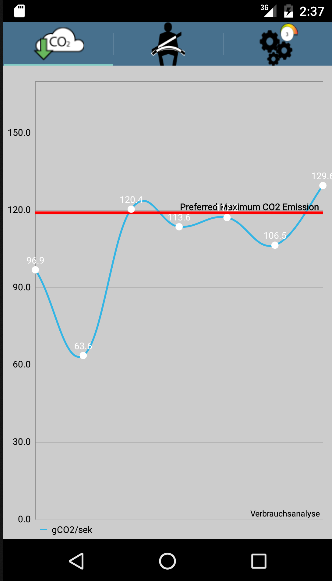
\includegraphics[width=0.3\textwidth]{images/verbrauch}
    \caption{Die Implementierung der Verbrauchsanalyse \cite{BOZH.ch3-verbrauchsanalyse.verbrauch}}
\end{wrapfigure}

Die Implementierung der Verbrauchsanalyse ist in Form eines dynamischen Liniendiagrammes erfolgt.
Mit der Library MPAndroidChart ist es uns gelungen, unser Liniendiagramm dynamisch zu gestalten.
Das bedeutet, dass sich nach einer gewissen Zeit, die Aktivität selbst aktualisiert.
Um den Benutzer während der Fahrt nicht mit unnötigen Informationen zu beladen, wurden die graphischen Elemente innerhalb der Applikation schlicht gehalten.\nextline
Während der Fahrt fokussiert sich der Benutzer von BestShift darauf, die rote Begrenzungslinie nicht zu überschreiten.
Somit erzielt man auf kurzer Dauer einen geringeren Kraftstoffverbrauch.


\clearpage % DO NOT REMOVE